\documentclass[twocolumn,10pt]{ltjsarticle}

\usepackage[top=20mm,bottom=20mm,left=25mm,right=25mm,columnsep=10mm]{geometry}
\usepackage[haranoaji,nfssonly]{luatexja-preset}
\usepackage{graphicx}
\usepackage{titlesec}
\usepackage{url}

\titleformat*{\section}{\Large\bfseries}
\titleformat*{\subsection}{\large\bfseries}

\title{【調査】感染症の接触段階における有効な追跡技術}
\author{山下 尚彦}
\date{\today}

\begin{document}
\maketitle

\section{はじめに}
2020年、特に3月以降から新型コロナウイルス(COVID-19)の脅威が世界中に広まり\cite{外務省2020感染状況}, 
その特徴として潜伏期間が長いことが挙げられる. そのため, その間に接触した人が感染する可能性があり, 今日のような
COVID-19感染者が爆発的に増えていると考えられる. 
そこで, 欧州の8大学を中心としたアカデミアグループが進めるプロジェクトDP-3T\cite{GitHub2020DP3Tdoc}では, 
スマートフォンなどのデバイスを利用して感染者と接触した可能性のある人を追跡し, 
接触者に対する通知プロセスを迅速・簡略化することで新型コロナウイルスの拡散を遅らせる技術を提案した. 
また, CoEpi, CovidWatch, Zcash Foundationの3グループが実装した
TCN Protocol\cite{GitHub2020TCNProtocol}やMITが提案した
PACT Protocol\cite{Ronald2020PACT}のいずれもBluetoothの機能を利用して感染者との接触した人の特定を行っている. 
これらの技術ではデバイスやユーザ, 位置などのセンシティブな情報は利用しないため, プライバシーの問題を解決する事ができる. 
次の章からTCN Protocolを例にその仕組みを説明する. 

\section{概要}
TCN ProtocolはTemporary Contact Numbersの頭文字から由来しており, 一時的な疑似乱数値を用いることで
プライバシーに配慮して接触者を追跡するプロトコルである. 

\subsection{プライバシーとセキュリティの保証}
感染者を追跡する情報を扱ううえでプライバシーなどの課題が挙げられる. 
TCN Protocolのプロジェクトでは, 追跡技術のプロトコルにおけるプライバシーとセキュリティを保証するには
以下の性質が望ましいとしている. 

\begin{description}
    \item[\textbullet サーバに対するプライバシー]~\\
    サーバはユーザの位置情報などの個人情報を取得しない
    \item[\textbullet ソース情報の完全性]~\\
    ユーザは接触していないユーザにレポートの送信や, 他のユーザの代わりにレポートを送信しない
    \item[\textbullet ブロードキャストにおける完全性]~\\ 
    ユーザーは自身が生成していない擬似乱数値をブロードキャストしない
    \item[\textbullet ソース情報のセキュリティ]~\\ 
    悪意あるユーザがレポートを送信していないユーザに関する情報を取得できないようにする
    \item[\textbullet レポート受信者に対するプライバシー]~\\ 
    レポートを受け取ったユーザが第三者にその情報を公開できないようにする
    \item[\textbullet レポート送信者に対するプライバシー]~\\ 
    レポートを送信するユーザは接触者にのみ接触した時間の情報を開示する
\end{description}

\subsection{接触者の追跡方法}
接触者の追跡は以下のフェーズによって行われる. 

\begin{description}
    \item[\textbullet ブロードキャスト]~\\
    疑似乱数値を生成して近くのデバイスにブロードキャストする
    \item[\textbullet レポート]~\\
    COVID-19に感染した場合, 潜伏期間中に接触した可能性のあるユーザを把握するためにサーバにレポートを送信する
    \item[\textbullet スキャン]~\\ 
    COVID-19の感染者に接触した可能性があるかサーバに問い合わせる
\end{description}

疑似乱数値のブロードキャストにはBluetooth Low Energy(BLE)を利用できるiOSおよびAndroid OSの機能を
用いるため, 異なるOS間であっても疑似乱数値の送受信は可能である. 
感染者は潜伏期間の範囲と疑似乱数値を計算するための鍵, 署名の検証鍵をサーバに
送信することで, サーバは感染者が潜伏期間中に他ユーザにブロードキャストした疑似乱数値を計算する. 
他ユーザは, 感染者から受け取った疑似乱数値を保持していないかサーバに問い合わせることで, 自身が接触者か確認できる. 

\section{TCN Protocolによる追跡}
接触者の追跡には, 疑似乱数値を生成して近くのデバイスにブロードキャストするブロードキャストフェイズ, 
感染者がサーバにレポートを送信するレポートフェイズ, 自身が接触者になっているかを確認するスキャンフェイズがあり, 
それぞれの詳しい仕組みを次の節より示す. 
以下はTCP Protocolで登場する鍵と擬似乱数値を表す用語である. 

\begin{description}
    \item[\textbullet RAK(Report Authorization Key)]~\\
    レポートの署名を行う秘密鍵
    \item[\textbullet RVK(Report Verification Key)]~\\
    レポートの検証を行う公開鍵
    \item[\textbullet TCN(Temporary Contact Number)]~\\
    Bluetoothでブロードキャストされる疑似乱数値
    \item[\textbullet TCK(Temporary Contact Key)]~\\
    TCNを計算するための値
\end{description}

\subsection{ブロードキャストフェイズ}
ブロードキャストフェイズの初期段階として, 署名に使用する鍵ペアRAK, RVKの作成と
疑似乱数値TCNを計算するTCKの初期値${TCK_0}$の作成がある. 
その後, ${TCK_0}$とRVKのハッシュ値から${TCK_1}$を求め, ${TCK_1}$から${TCN_1}$を計算し, 
その値をBluetoothを介して他ユーザにブロードキャストする. 
${TCN_1}$以降のTCN(${TCK_n (n > 0)}$)は, ${TCN_{n-1}}$とRVKのハッシュ値から計算される. 
実際の実装でのTCKは, 自身のインデックスを表す${index}$とRVKを保持する${rvk}$, 
${TCK_{n-1}}$とRVKのハッシュ値から求められた${bytes}$を持つ構造体である. 
${TCK_1}$のそれぞれの値の計算式を以下に示す. 
また, \textbf{図\ref{fig:calc_tcn}}は疑似乱数値TCNを計算する手順を表したものである. 

\begin{eqnarray*}
    && index = TCK_{n-1}.index + 1 \\
    && rvk = TCK_{n-1}.rvk \\
    && bytes = H(TCK_{n-1}.rvk, TCK_{n-1}.bytes)
\end{eqnarray*}

\begin{figure}[htb]
    \centering
    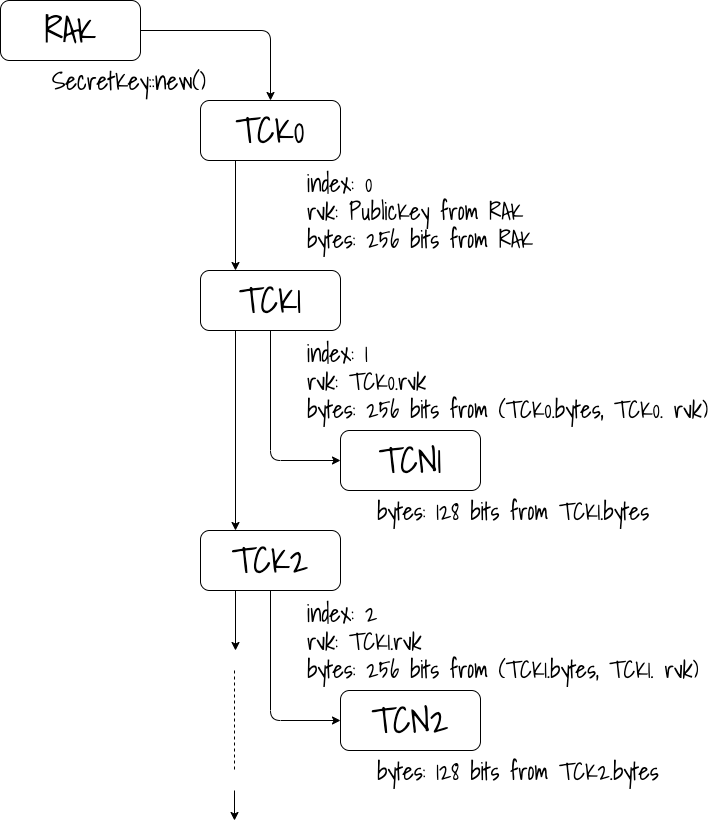
\includegraphics[width=6cm]{images/【調査】感染症の接触段階における有効な追跡技術/TCNProtocol.png}
    \caption{TCNを計算する手順}
    \label{fig:calc_tcn}
\end{figure}

\subsection{レポートフェーズ}
RVKと${TCK_i}$をレポートとしてサーバに送信することで, ${TCK_i}$以降の${TCK_j}$と
${TCN_j}$(${j \geq i}$)を計算することができるので, すべてのTCKを送信する必要はない. 
感染者の潜伏期間と思われる期間を${(j_1, j_2)}$とする. 
ユーザはレポートを送信する際に, ${RVK}$, ${TCK_{20}.bytes}$, ${j_1}$, ${j_2}$の4つの情報を送信することで, 
サーバ側で${RVK}$と${TCK_{20}.bytes}$から${(TCN_{20}..TCN_{90})}$を計算できる. 

\subsection{スキャンフェーズ}
他ユーザはサーバにアクセスすることで, 自身が感染者のTCNを保持していないかを確認することで
感染者と接触したかを判断できる. 

\section{おわりに}
TCN Protocolを利用することで位置情報などの個人情報を必要としないで接触者を追跡でき, 
感染経路の特定が容易にできると考えられる. 
ただし, このプロジェクトではTCKの更新タイミングなどを言及していなかったため, どの程度の間隔でTCNをブロードキャストする
ことで追跡に有効なのかはわからなかった. 
また, 完全な乱数を生成することができないため接触者でない場合でも接触者と判断される可能性がある. 
さらに, 保健所が実際にこのような技術を導入した際には時間や個人を特定するために
個人情報等をサーバに送信する必要があるため, 新たにプライバシーの問題が発生すると考えられる. 

\bibliographystyle{junsrt}
\bibliography{DB}
\end{document}